


\documentclass[11pt]{article}

\usepackage[utf8]{inputenc} 
\usepackage[T1]{fontenc} 
\usepackage{graphicx}
\usepackage{grffile}
\usepackage{mathpazo} 
\usepackage{indentfirst}
\usepackage[section]{placeins}
\usepackage[hyphens]{url}
\usepackage{hyperref}
\usepackage{xcolor}
\hypersetup{
    colorlinks,
    linkcolor={red!50!black},
    citecolor={blue!50!black},
    urlcolor={blue!80!black}
}
\PassOptionsToPackage{hyphens}{url}\usepackage{hyperref}[hidelinks]


\begin{document}



%----------------------------------------------------------------------------------------
%	TITLE PAGE
%----------------------------------------------------------------------------------------

\begin{titlepage}
	\newcommand{\HRule}{\rule{\linewidth}{0.5mm}} 
	
	\center
	
	%------------------------------------------------
	%	Headings
	%------------------------------------------------
	
	\textsc{\LARGE Université Paris Dauphine}\\[1.5cm] 
	
	\textsc{\Large Master 1 MIAGE}\\[0.5cm] 
	

	
	%------------------------------------------------
	%	Title
	%------------------------------------------------
	
	\HRule\\[0.4cm]
	
	{\huge\bfseries Projet d'Analyse et Fouilles de Données}\\[0.4cm]
	
	\HRule\\[1.5cm]
	
	%------------------------------------------------
	%	Author(s)
	%------------------------------------------------
	
	\begin{minipage}{0.4\textwidth}
		\begin{flushleft}
			\large
			\textit{Réalisé par :}\\
			Lyes \textsc{MEGHARA}\\ 
			Kamel \textsc{SIDHOUM}\\ 
		\end{flushleft}
	\end{minipage}
	~
	\begin{minipage}{0.4\textwidth}
		\begin{flushright}
			\large
			\textit{Encadré par :}\\
			Mr Yann \textsc{CHEVALEYRE}% Supervisor's name

		\end{flushright}
	\end{minipage}
	

	
	
	\vfill\vfill 
	
	{\large18 Mai 2017} 
	



	\leavevmode \newline 	\leavevmode \newline 	\leavevmode \newline 	\leavevmode \newline 	\leavevmode \newline 
	
\includegraphics[width=0.6\textwidth]{dauphine.png}\\[1cm] 
	 

	

	
\end{titlepage}

\renewcommand{\thesection}{\Roman{section}}
\renewcommand{\thesubsection}{\thesection.\Roman{subsection}}





\section{Introduction}


La notion d'apprentissage supervisé a été évoquée depuis plus de cinquante ans. Cela a permis l’évolution concrète de l’intelligence artificielle au plus grand bonheur des informaticiens et étudiants. Le projet que nous allons exposer traite de la capacité de plusieurs algorithmes d’apprentissage supervisé à apprendre, puis à prédire. \newline  \newline
Nous disposons pour cela d’une base de données fournie par \textsc{litislab} dans le contexte d'une compétition nommée « \textit {My Tailor is rich!} » composée de plusieurs milliers de textes en Anglais, chacun possédant des variables numériques prédictives, et la variable à prédire (i.e le niveau). \newline \newline
Notre objectif est d'établir un (voir plusieurs) classifieurs à partir de cette base de données. Nous allons répartir les données en deux ensembles, un sur lequel notre (nos) classifieur va \textit {« apprendre »} et un autre ensemble sur lequel il va pouvoir \textit {« prédire» } le niveaux d'Anglais.\newline 


\section{Outils de développement}

Dans le cadre de ce projet, nous avons utilisé GitHub pour une meilleure collaboration, Jupyter Notebook avec les librairies Keras et Scikit-Learn \newline Pour finir ce rapport a été rédigé en utilisant LateX.

\section{Première approche}

\subsection{Prétraitement}

Une première approche a consisté a utiliser un réseaux de neuronnes artificiels et multiclasse pour procéder à l'apprentissage puis à la prédiction, mais avant cela un prétraitement  (dite de preprocessing) des données était un passage obligatoire, en effet, les données ont plusieurs valeurs manquantes, tels que les NaN (Not a Number). \newline
Après avoir remplacé ces dernières par des 0, il a fallu centrer-réduire les données c'est là que StandardScaler() nous a été utile.  \newline
Enfin, puisque les variables à prédire sont nominales (Niveaux allant de A1 à C2) il a fallu les encoder via L'Encodage one-hot, puis les transformer en valeurs numériques.\\
Il est à noter, que cette première approche ne tient pas compte du texte, mais uniquement des variables numériques.

\subsection{Construction du modèle}

Une fois le prétraitement terminé, on découpe notre modèle en deux sous ensembles X\_train et X\_test avec une répartition de 60\%, 40\% . \newline

Après plusieurs recherches et tests, nous avons opté pour le modèle \textit{Sequential} de Keras, celui ci permet de paramétrer le réseau couche par couche sans trop de difficulté. \newline \newline
Comme citée lors du dernier cours, la fonction d'activation \textit{Relu} a donné de bien meilleurs résultats comparé à la fonction \textit{Sigmoid}.\\ Nous avons donc opté pour un réseau à 3 couches et c'est donc dans les deux premières couches (input et hidden) que notre choix s'est porté sur \textit{Relu}. \newline \newline
En revanche, pour la dernière couche (output), d'après nos recherches puis, nos tests; il s'avère que la fonction d'activation \textit{Softmax} ainsi que la fonction de perte \textit{Categorical\_crossentropy} étaient plus adaptés pour des classes multiples. \newline


\subsection{Résultats des tests}


Après plusieurs paramétrages, on constate qu'avec 100 itération, on arrive à des résultats très satisfaisants. Notre taux d'erreurs se situe entre 3\% et 5\% \newline \newline

\begin{figure}[!htb]
  \centering
    \caption{Evaluation du modèle}
    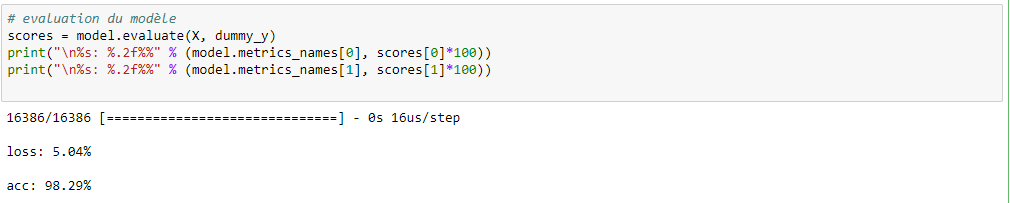
\includegraphics[width=\textwidth]{loss.png}
    \end{figure}
    



\begin{figure}[!htb]
Les prédictions sur X\_test comparé aux valeurs réelles Y\_test sont exposées sur les 2 figures suivantes : \\
  \centering
    \caption{Prédictions sur X\_test}
    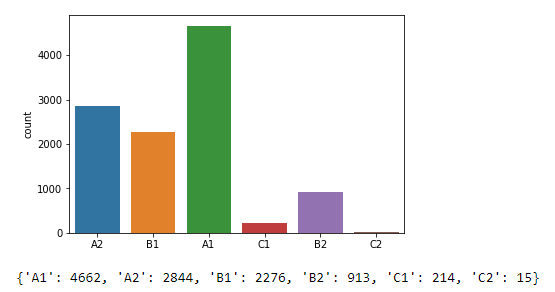
\includegraphics[width=\textwidth]{predictions.png}
	\textit {Effectifs prédits par classe}
\newline \newline

  \centering
    \caption{Les valeurs réelles}
    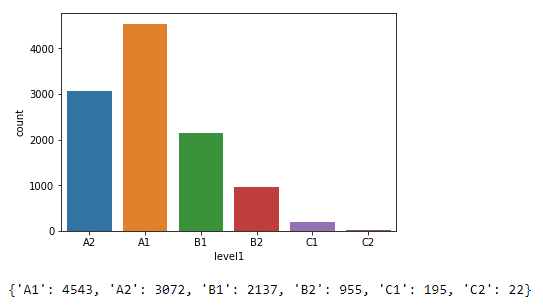
\includegraphics[width=\textwidth]{relles.png}
	\textit {Effectifs réels par classe}

\end{figure}

\section{Autres Classifieurs}

Cette fois-ci, en utilisant la librairie Scikit-Learn, on a pu tester et comparer divers classifieurs entre eux. \newline
Les classifieurs testés sont : Régression Logisitque, Arbre de décision, KNN, LDA, Random Forest et d'autres encore. \newline  \newline
Sans surprise, comme notre enseignant Mr Chevalyere nous l'avait recommandé, Le Random Forest est bien plus performant que les autres. \newline   \newline
KNN aussi se démarque bien, mais comme il ne construit pas de modèle et est obligé de charger tout en mémoire à chaque lancement, ce dernier est bien plus lent que les autres. \newline\newline
Tous les résultats détaillés sont consultables sur le fichier \textit{ManyClassifiers.ipynb}


\begin{table}[h!]
  \begin{center}
    \caption{Précision par classifieur}
    \label{tab:table}
    \begin{tabular}{c c c c c c} % <-- Alignments: 1st column left, 2nd middle and 3rd right, with vertical lines in between
      \textbf{Regression Logistique} & \textbf{Arbre de décision} & \textbf{KNN}   & \textbf{LDA}  & \textbf{Bayes Naif}  & \textbf{Random Forest}\\
      \hline
       0.72\% & 0.72\%  & 0.77\% & 0.73\% &  0.66\% & 0.78\% \\ 
    \end{tabular}
  \end{center}
\end{table}


\section{KMeans}

Bien que le Clustering, et plus particulièrement KMeans ne soit pas une méthode d'apprentissage supervisée, mais plutot non supervisée, nous avons voulu tester et voir les résultats par nous meme, et ce en faisant abstraction de la variable à prédire (le niveau). \newline \newline
Nous nous basons sur k=6, (6 clusters, car 6 niveaux différents),  les résultats obtenus sont présentés dans les figures suivantes : \newline

\begin{figure}[!htb]
  \centering
    \caption{Nuage de points au début}
    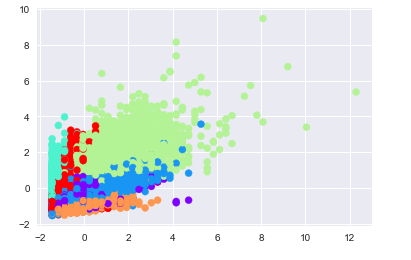
\includegraphics[width=\textwidth]{kmeansdeb.png}


  \centering
    \caption{Nuage de points après 50 étapes}
    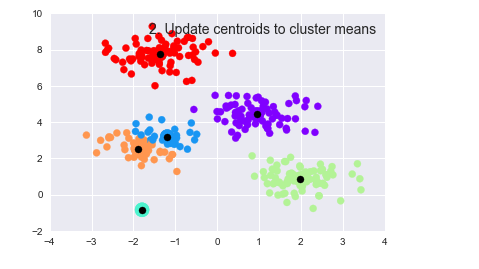
\includegraphics[width=\textwidth]{kmeansfin.png}


\end{figure}


\section{Seconde approche}

\subsection {Introduction}

Dans cette partie nous allons analyser uniquement la partie texte, soit la colonne « fulltext » ainsi que la classification qui leurs sont associées.
La classification de texte est utilisée dans différent domaine, que cela soit pour définir les sentiments émis par un texte, filtrer les « spams » etc…
Notre but ici est donc d’assigner un texte à un des 6 classifications, nous ferons ici l’hypothèse que chaque texte sera associé à une et une seule catégorie. 

\subsection {Prétraitement}

Dans notre cas, nous aurons en entré les textes en anglais \textit{« fulltext »} et en sortie le niveau correspondant \textit{« level1 »}. \newline
Nous avons aussi créé une colonne nommée \textit{« category\_id\_df »} codant les niveaux d’anglais par un entier (de type Integer) car les variables sont souvent mieux représentées par des entiers que par des chaines de caractère.\newline \newline

\begin{figure}[!htb]
  \centering
    \caption{Tableau représentant les textes selon leurs niveaux et catégories}
    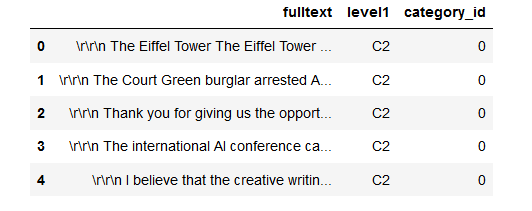
\includegraphics[width=\textwidth]{textmining.png}
\end{figure}

Il faut savoir que les classifieurs ainsi que les algorithmes d’apprentissage n’arrivent pas à traiter directement du texte brut, ils s’attendent à recevoir des vecteurs de caractéristiques numériques, on convertit donc durant cette phase les textes en entiers.\newline \newline
Une approche simple pour essayer d’extraire les caractéristiques d’un texte est tout simplement d’utiliser ce qu’on appelle communément \textit{« a bag of words model »}, soit un modèle pour chaque texte où la fréquence d’apparition des mots est prise en compte et l’ordre des mots n’importe peu et donc nous obtenons pour chacun des 27 310 textes un total de 12 633 caractéristiques représentant le score pour différent unigram  et bigram.\newline
En utilisant la bibliothéque \textit{« Sklearn »}  cela nous donne accès à des fonctions pouvant faire un lien entre des termes et des niveaux d’anglais, ici nous avons choisi d’afficher deux unigrams et deux bigrams qui sont le plus corrélés à chaque niveau, nous obtenons : 

\begin{figure}[!htb]
  \centering
    \caption{Tableau représentant des unigrams et des bigrams selon le niveau}
    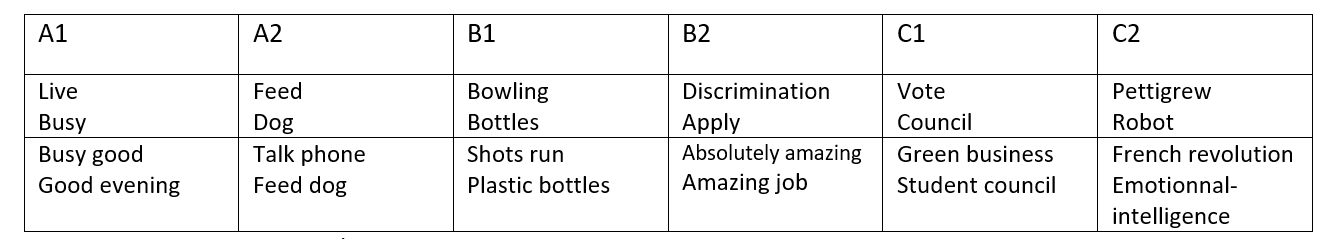
\includegraphics[width=\textwidth]{texttab.png}
\end{figure}

\subsection {Construction du modèle}

Après quelques recherches, nous nous sommes penchés sur le modèle \textit{« LinearSVC »} donnant des résultats extrêmement satisfaisant, même meilleur que l’algorithme de \textit{« RandomForest »}, beaucoup de données sont affichés dans le programme \textit{Etude-de-Texte.ipynb }, notamment la matrice de confusion ainsi que des tableaux montrant des erreurs de prédictions soit comment certains textes sont catégorisés dans un niveau qui n’est pas le leur. \newline
\begin{figure}[!htb]
  \centering
    \caption{Nous obtenons donc comme résultat }
	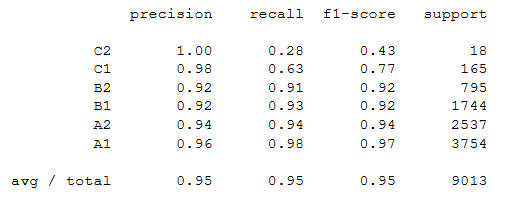
\includegraphics[width=0.9\columnwidth]{textresults.png}
\end{figure}

\clearpage

\section{Webographie} 
\begin{itemize}
\item \url{https://medium.com/@pushkarmandot/build-your-first-deep-learning-neural-network-model-using-keras-in-python-a90b5864116d} \newline
\item \url{https://machinelearningmastery.com/tutorial-first-neural-network-python-keras/} \newline
\item \url{https://towardsdatascience.com/deep-learning-gender-from-name-lstm-recurrent-neural-networks-448d64553044} \newline
\item \url{https://towardsdatascience.com/multi-layer-neural-networks-with-sigmoid-function-deep-learning-for-rookies-2-bf464f09eb7f} \newline
\item \url{https://machinelearningmastery.com/multi-class-classification-tutorial-keras-deep-learning-library/} \newline
\item \url{https://towardsdatascience.com/solving-a-simple-classification-problem-with-python-fruits-lovers-edition-d20ab6b071d2} \newline
\item \url{https://www.kaggle.com/mjamilmoughal/k-nearest-neighbor-classifier-to-predict-fruits} \newline
\item \url{https://towardsdatascience.com/multi-class-text-classification-with-scikit-learn-12f1e60e0a9f} \newline
\item \url{http://blog.aylien.com/first-text-mining-project-python-3-steps/} \newline
\item \url{https://www.digitalvidya.com/blog/an-introduction-to-text-analysis-in-python/} \newline
\item \url{https://fr.wikipedia.org/wiki/Encodage_one-hot/} \newline

\end{itemize}

\end{document}
